\chapter{Conclusion}

%\begin{center}
%    \begin{CJK*}{UTF8}{gbsn}
%        \large 工欲善其事,必先利其器。\\[0.5em]
%        \small \hfill --- 《论语$\cdot$卫灵公》(春秋) \\ [0.8em]
%        \large A craftsman who wishes to perfect his work must first sharpen his tools. \\ [0.5em]
%        \small \hfill --- \textit{The Analects of Confucius $\cdot$ Wei Ling Gong} (circa 475-400 BCE)
%    \end{CJK*}
%\end{center}

% wider than default
\setlength{\epigraphwidth}{0.5\textwidth} 
\begin{CJK*}{UTF8}{gbsn}
    \epigraph{
        工欲善其事,必先利其器。\\
        A craftsman who wishes to perfect his work must first sharpen his tools.
    }{
        ---《论语$\cdot$卫灵公》(春秋)\\
        --- \textit{The Analects of Confucius$\cdot$Wei Ling Gong} \\
        (c. 475-400 BCE)
    } 
\end{CJK*}


As the above saying goes, effective work requires well-prepared tools. In modern society, engineering design serves as a cornerstone of manufacturing and production.

Traditional engineering design remains a labor-intensive, costly and domain-fragmented process. This thesis began with the observation that realizing high-performance designs, such as aerodynamic shapes, still requires extensive human effort across multiple specialized tools and disciplines. While prior AI research promises to accelerate certain design steps, these approaches are imperfect: many are data-hungry, requiring prohibitive datasets; and their workflows are opaque black boxes that are less robust, controllable and explainable to users.

To address these challenges, this thesis set a clear goal: to fully augment engineering design, we need structured AI-driven methods that integrate tightly with physics, use data efficiently, and remain controllable. The proposed solution built on deep geometric learning techniques and was twofold: (i) develop differentiable shape representations and automated geometry models to drive optimization, and (ii) create data-efficient, controllable generative models to drive exploration; with both aspects guided by physics and geometric constraints. By combining these elements, the work aimed to transform the design process from a slow, expert-dependent sequence into a more automated, compact workflow where human engineers team with AI to accelerate and scale up.

\section{Summary of Contributions}

To realize the above visions, this thesis addressed five key research questions (Q1–Q5) outlined in Chapter~\ref{ch1:sec:scopes}.

\textbf{Q1 Representation:} A differentiable latent representation (Chapter~\ref{ch3}) and a self-prior, network-based representation (Chapter~\ref{ch5}) are developed for aerodynamic shapes that spans both the surface geometry and the volumetric computational mesh. Both learned representations ensure that shape modifications remain smooth and simulation-ready, allowing gradients from physics solvers to propagate directly into shape updates.

\textbf{Q2 Parameterization Choice:} Chapter~\ref{ch4} compares two automatic parameterizations: a \emph{Latent Space Model} (LSM) learned from data and a \emph{Direct Mapping Model} (DMM) constructed without reliance on a training set. Both eliminate manual intervention typical of handcrafted parameterizations and achieve performance on par with those baselines in 2D airfoil optimization. However, their strengths differ in useful ways: the LSM leverages its dataset prior to provide a well-conditioned latent space with a built-in sampling capability for generating valid airfoils. In contrast, the DMM can develop shape patterns not present in existing profiles and thus can provide task-oriented improvements even outside any observed distribution. Meanwhile, Chapter~\ref{ch4} introduce a mesh-free, simplified, and generic regularization that learns continuous coordinate mappings, which makes computational mesh deformation more robust across cases. In summary, Q2 is answered by showing that both models are effective for design quality while offering complementary advantages and flexible, reliable mesh-deformation handling.

\textbf{Q3 Automating Design Optimization at Scale:} Building on the above conclusions, this thesis introduces DeepGeo, a deep geometric mapping model that extends the prior DMM. DeepGeo replaces the laborious, hand-tuned setup of conventional methods with a trainable neural parameterization, with a special focus on scaling to complex configurations. Chapter~\ref{ch5} addresses Q3 through three test cases: (i) DeepGeo optimizes a 2D circle, producing a shape exhibiting transonic airfoil characteristics, which were previously intractable with conventional Free-Form Deformation techniques; DeepGeo successfully optimizes a business-jet wing; and (iii) a full aircraft wing–body configuration, both with state-of-the-art performance. Notably, all cases use the same configuration, methodology and hyperparameters as in the first 2D task. These results underscore DeepGeo’s role as an automated, scalable geometry model for high-dimensional and high-fidelity design optimization.

\textbf{Q4 Generative Exploration:} While DeepGeo focuses on improving an existing design via optimization, this thesis also tackles the complementary challenge of exploring entirely new design shapes. To this end, Chapter~\ref{ch6} introduces DiffGeo, a latent diffusion generative model for novel shape sampling. DiffGeo learns a probability model in the same compact latent space that encodes valid shapes, enabling it to generate new aerodynamic shapes that are both diverse and valid by construction. Notably, DiffGeo was designed to be data-efficient and controllable. The generated candidates exhibited a rich diversity comparable to those from GANs or VAEs trained on orders of magnitude more data, and almost all samples respected basic design constraints. This contribution answers Q4 by demonstrating a viable approach to exploratory design generation: engineers can use DiffGeo to quickly produce a breadth of design alternatives for inspiration or further analysis, rather than relying on intuition or brute-force search.

\textbf{Q5 Physics-Guided Generation:} The final research question extends the generative approach by asking whether physics knowledge can be injected into the generation process without retraining the generator. To address it, Chapter~\ref{ch7} developed a model termed Dfow-SUR, where surrogate gradients guide the DiffGeo sampler during inference, effectively inducing unconditional generations with domain knowledge. Chapter~\ref{ch7} shows that Dfow-SUR can significantly improve the likelihood of satisfying specified aerodynamic criteria in generated shapes comparing to prior studies in generation controls. Notably, this guidance does not require modifying or retraining the generative model itself, and the same pretrained DiffGeo model can be re-used for different objectives by simply plugging in the appropriate physics-based energy during sampling. In summary, Q5 is addressed by demonstrating physics-guided generative design: an approach that combines the creativity of generative models with the rigor of physics-based optimization, allowing engineers to control automatic design generation toward feasible, high-performance solutions in a flexible and computationally efficient manner.

\section{Future Work and Outlook}

\begin{figure}[!t]
    \centering
    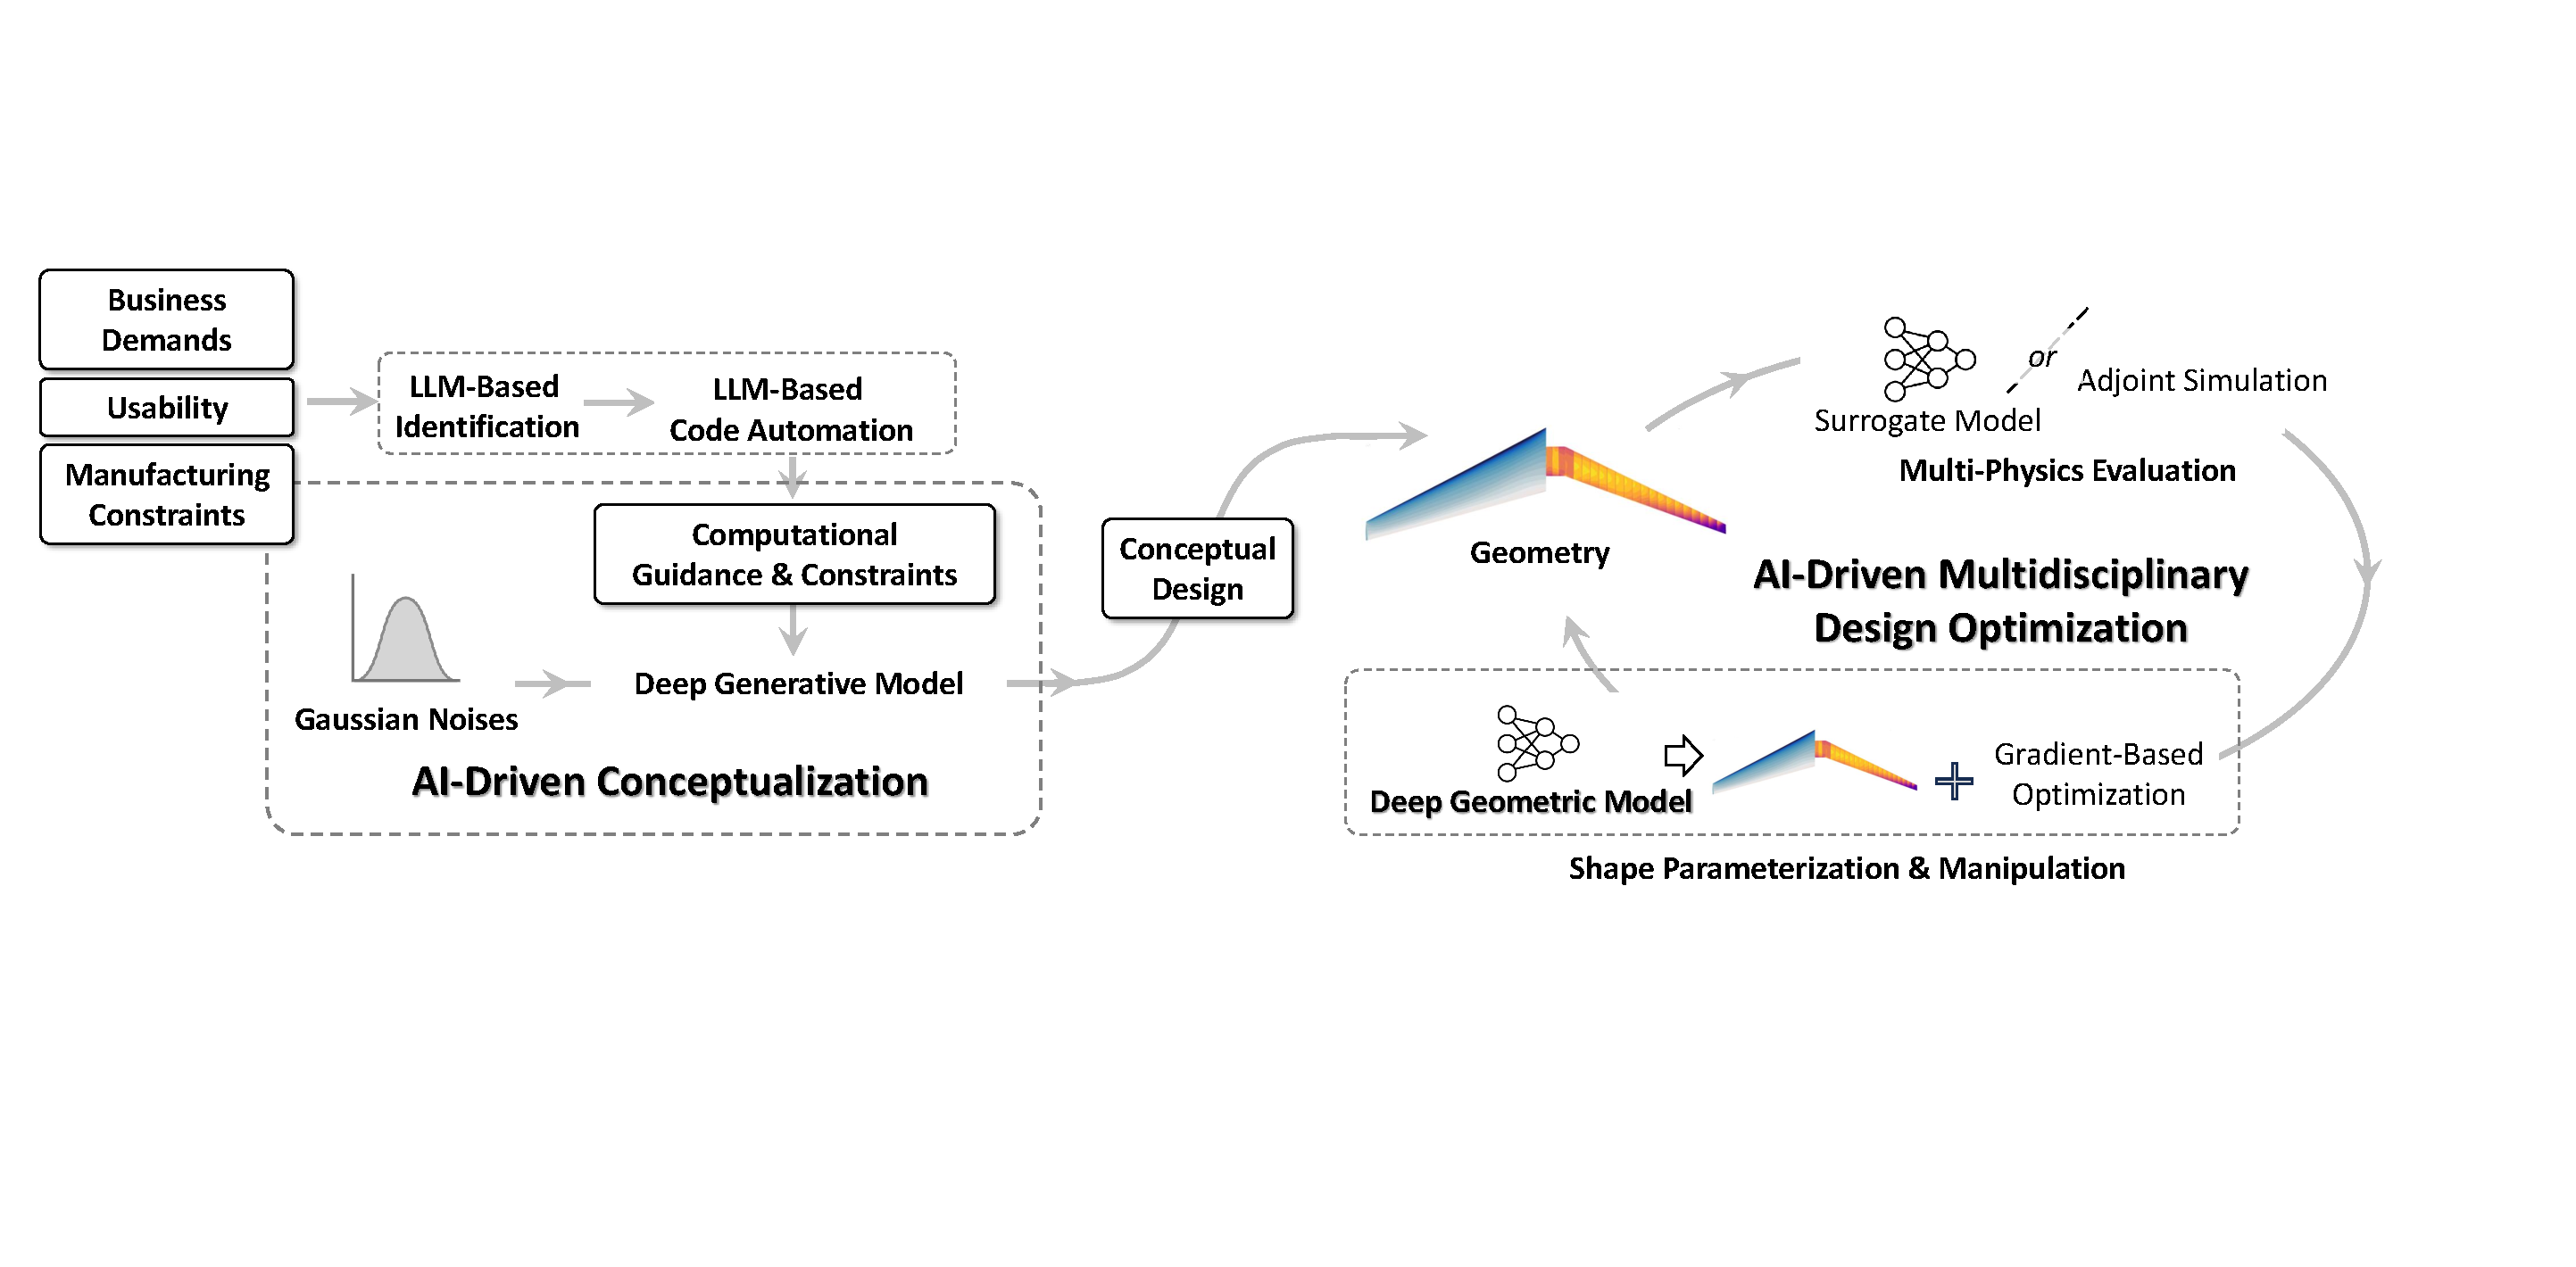
\includegraphics[width=1\linewidth]{conclusion/fig/future_work.pdf}
    \caption{Future working directions toward a fully AI-driven Model-Based Engineering pipeline, integrating LLM agents, generative conceptualization and automated multidisciplinary optimization with deep geometric parameterization.}
    \label{conclusion:fig:future_work}
\end{figure}

While this thesis has made progress toward AI-augmented design, it also opens several promising directions for future investigation. I aim to pursue an AI-driven Model-Based Engineering platform that unifies Generative Models (GenM) for conceptual exploration, Geometric Models (GeoM) for high-fidelity optimization, and Large Language Model (LLM) agents for design identification and code automation. The overall goal is a modular, data-efficient and physics-guided workflow that embeds manufacturability, robustness and regulatory compliance directly into the computational constraints of automated design space exploration and optimization. 

The first working direction will extend DiffGeo and Dfow-SUR with multi-physics energy guidance, enabling exploration of feasible concept spaces under explicit physical and Design-for-Manufacturing (DfM) constraints, while providing uncertainty-aware and diversity-controlled design proposals. The second working direction will further develop DeepGeo for multidisciplinary, multi-fidelity and multi-point optimization, with enhanced robustness and integrated uncertainty quantification. The third working direction will leverage LLM-based design agents to translate natural-language requirements and standards into executable, verified constraint code, thereby reducing human–AI interaction barriers and enhancing the usability of the design framework. As illustrated in Figure~\ref{conclusion:fig:future_work}, these components will be seamlessly integrated into a more automated and robust framework, with sufficient modularity and controllability to democratize advanced CAD/CAE techniques and shape the future of engineering design.